\section{Define the Problem of Mapping the Software Applications}\label{sec_problem}
The software applications are deployed on the execution platform in such a way that the user-defined requirements of the software applications such as the reliability requirements, end-to-end timing requirements, and criticality of the applications are satisfied. It is conducted by mapping the software-components replicas (or components in short) effectively on the computing nodes and the network bus, that is that is $\bigcup {\sss{Q}}\mapsto M'$, so that the total power consumption $Power(\textbf{x})$ of the applications is minimized. The latter  is achieved by selecting nodes that consume lower power $M'\subseteq M$, provided that the reliability of each application $Reliability_a(\x)$, the timing $ResponseTime_\tau(\x)$, $Delay_\gamma(\x)$, and placement constraints fullfill respective software applications requirements.It is a type of Job Shop scheduling with constraints, as such, it is a discrete optimization problem. 

The solution to the allocation problem is represented by a vector-matrix $\x=\{\xsp{A_k}:k=1,...,N_a\}$ as shown in Equation (\ref{eqn_solution}), where \ttxsp{k} is a matrix of size $n_C\times K$, and \ttssx{x}{k}{ij}$=h\in \{1,…,n_N\}$ denotes the mapping of the  software-component replica \ttssx{q}{k}{i,j} to the computating node $n_h$.
\begin{equation}
\label{eqn_solution}
\bspx{k}=
\begin{bmatrix} 
\ssx{k}{11} & \ssx{k}{12} & \dots & \ssx{k}{1K}\\
\ssx{k}{21} & \ssx{k}{22} & \dots & \ssx{k}{2K}\\
\vdots & \vdots & \ddots & \vdots\\
\ssx{k}{N_c1} & \ssx{k}{N_c2} & \cdots & \ssx{k}{N_cK}
\end{bmatrix}
\end{equation}

The formulation of the power consumption and timing depends on the tasks graphs $\bigcup\sss{g}[k][\tau](\x)$, which are a function of the mapping \ttx. However, if the tasks graphs are apriori to the software allocation problem, the formulation of a task graph is not necessary. Note: the latter is true if no runnables from different components map to a single task, in this case, the tasks graphs are independent of \ttx. The task graph formulation is shown in the next subsection.

\subsection{Task Graph Formulation}
The task graph formulation implies the generation of a task graph, with the cost of the tasks nodes and the links updated for the mapping \ttx. The tasks nodes are updated with the timing information and the mapping to computing nodes, likewise, the links with the mapping on the bus (1 if mapped on the bus, 0 otherwise). The formulation has two steps: i) for a mapping \ttx , we update the runnables with nodes information to which they are mapped by traversing elements of the mapping \ttx, $\xkij$, in linear-time complexity $O(n)$, where $n=|\x|*n_r$, and $n_r$ is the  runnables per software component using Equation (\ref{eqn_uprdaterunnables}); ii) by applying the merging rules, we traverse the runnables graphs in the system and subsequently generate the tasks graphs using Equation (\ref{eqn_generatetasksgraphs}).
\begin{align}
\label{eqn_uprdaterunnables}
&\forall k,ij\ \forall r\in V(\sss{g}[k][])\ node_r = n_h& \mbox{, where } h=\xkij\\
\label{eqn_generatetasksgraphs}
&\forall k\ \sss{g}[k][r](\x)\xrightarrow{\text{Eqn. (13);Merging Rules}}\sss{g}[k][\tau](\x)
\end{align}

where $V(\sss{g}[k][])$ returns the runnables nodes of the graph $\sss{g}[k][]$.

\subsection{Total Power Consumption}
%where $P_{m}(\textbf{x})$ is the power consumption of a  computing node $m$ with the mapping $\textbf{x}$. 
%$Power(\textbf{x})=\sum_{m\in M'}{P_{m}(\textbf{x})}$
%Power consumption refers to the energy usage of electronic components in an integrated circuit, e.g., processor, memory, I/O devices, etc., per time unit. 
There are several models (or techniques) to estimate the power consumption of a computing node. In this work, we use a technique based on processor load (or utilization) to estimate the average power consumption of a computating node. Specifically, we use the linear polynomial model proposed by Fan et al. \cite{Fan2007PowerComputer}, which is shown in (\ref{eqn_powerconsumption}). The model states that the power consumption of a node is directly proportional to its load, and is inductively formulated from experimental results:
\begin{equation}
\label{eqn_powerconsumption}
f_p(u)=P_{idle} + (P_{busy}-P_{idle})*u,
\end{equation}

where $u$ is the utilization of a computating node, $p_{idle}$ and $p_{busy}$, respectively refer to the power consumption measured at minimum and maximum processor loads. Such measurements can be obtained by running performance benchmark suits, e.g., MiBench \cite{Guthaus2001MiBench:Suite}, AutoBench \cite{EMBC2018AutoBenchProcessors}, etc.

Subsequently, the power consumption of a node $m$ for a given mapping $\textbf{x}$ is formulated as follows: i) first using Equations (\ref{eqn_powerconsumption_x}-\ref{eqn_util_component}), by calculating first the node's utilization $U_m(\textbf{x})$ using Equation (\ref{eqn_util_x}). The node's utilization is computed from the set of components allocated to it (which are $\forall_{ij} x_{ij}=m$) using Equation (\ref{eqn_util_x}). And the utilization of a component on the node $m$ is computed from its constituent tasks $T_c$ using Equation (\ref{eqn_util_component}).
\begin{align}
	\label{eqn_powerconsumption_x}
nodPow(\textbf{x}) & =f_p(nodUti(\textbf{x},m))                         &  \\
	\label{eqn_util_x}
nodUtil(\textbf{x},m)           & = \sum_{k}{\sum_{i}{\sum_{j}{comUtil(m,c)}}}|\xkij=m         & \text{, where } c=\sss{C}\\
	\label{eqn_util_component}
comUtil(m,c)              & = \sum_{r\in c.R} \frac{r.e_m}{r.\tau.P}, &
\end{align}

where $c.R$ is set of runnables in component $c$, $r.e_m$ and $r.\tau.P$ are the execution of runnable $r$ on node $m$ and its period, respectively.

The applications requirements are modeled as constraints that need to be satisfied in the allocation problem. The constraints formulations are shown in the following subsections, respectively for reliability, timing and other design constraints such as related to runnables-to-tasks merging and replication.

\subsection{Software-Applications Reliability Constraints}\label{subsec_reliability_constraint}
The applications reliability constraints ensure the mapping $\textbf{x}$ satisfies the user-defined reliability requirements, that is $\forall k\ \rel_{A_k}(\x)\leq RelReq_{A_k}$. 
The reliability  is computed from the execution framework that is provided to run the application, which consists of computation nodes \ttssp{M} and the shared CAN bus B, as shown in Equation (\ref{eqn_appreliability_app}). The nodes host the components \ttssp{C} and are determined by searching the mapping \ttxsp{k}  in polynomial time using Equation (\ref{eqn_nodes_app}).
\begin{align}
	\label{eqn_appreliability_app}
	&Reliability_{A_i}(\x)=Reliability_{A_i}(\ssp{M})*Reliability(B)\\
	\label{eqn_nodes_app}
	&\ssp{M}=\{e|e\in M \land \forall ij (e=m_h) \},\mbox{ where } h=\ssx{k}{ij} 
\end{align}

The reliability of the nodes, $Reliability_{A_i}(\ssp{M})$ with respect to the application ${A_k}$ is calculated using the \textit{state-enumeration} technique \cite{Lucet1999ExactReliability}  as shown in Equations (\ref{eqn_appreliability}). According to the technique, the reliability is basically the total probability that the application $A_k$ \textit{functions} under mutually exclusive and uniformly distributed failure-events of the nodes, represented by $\ssp{\mathcal{F}}(\ssp{M})=\{\textbf{0},\textbf{1}\}^{\ssp{M}}$, where  \textbf{0} means node fails, \textbf{1} means  node is operational. An event $\omega\in \mathcal{F}_{A_k}(\ssp{M})$ represents the states of nodes by a sequence of 0-1 variables $(b_1,...,b_n)$, where $\omega.b_i$ denote the state of node $m_i\in \ssp{M}$. %as the state of the nodes $\ssp{M}=\{e_1,...,e_n\}$ by $s\in \ssp{\mathcal{F}}(\ssp{M})=(b_{e_1},...,b_{e_n})$, where $n=|\ssp{M}|$, whereas the state of a node is referenced by $s.b_{e}$.
\begin{align}
\label{eqn_appreliability}
Reliability_{A_i}(\ssp{M})&=\sum_{s\in \ssp{\mathcal{F}}|g(A_i, s)=1}probability(s)
\end{align}

The fact that an application functions $g(A_k, s)$ is defined via its inverse, which is \textit{software application failure}, deductively as follows:
\begin{definition}[Software Application Failure]
The application $A_k$ fails in the event $\omega \in \ssp{\mathcal{F}}(\ssp{M})$ if there exists a component type \ttsss{c} where all of its replica \ttsss{Q} \textit{fail}, otherwise, the application functions, as shown in Equation (\ref{eqn_app_failure}).  A component replica $\sss{q}[k][ij]\in \sss{Q}$ fails if the node that host it $m_h$ fails, where $h=\xkij$.  
\begin{align}
\label{eqn_app_failure}
g(a, \omega)&= 
\begin{cases}
\textbf{0} & \mbox{ if } \exists i\forall j\ (m_h\in \sss{M}[k][\omega] )\\
\textbf{1} & \mbox{ otherwise }
\end{cases}\\
\label{eqn_appreliability_node_s}
\sss{M}[k][\omega]&=\{e|e\in \ssp{M} \land (\omega.b_e=1) \},
\end{align}
\end{definition}
where \ttsss{M}[k][\omega] denote the nodes that function at the event $\omega$, and can be found by searching the nodes \ttssp{M} with state $\omega.b_e=1$ in constant time , as show in Equation (\ref{eqn_pro}).

The probability that a nodes-failure event $\omega$ occurs is computed as a product of the probabilities of its consitutuent elements $\omega.b$ as shown in Equation (\ref{label}).
\begin{equation}
\label{eqn_pro}
	\prod_{(m,b)\in (M,\omega)}{\lambda_m*(1-b)+(1-\lambda_m)*b}
\end{equation}
where $\lambda_m$ is the failure-rate of node $m$.

\subsection{Timing constraints}
The timing constraints ensure that the applications are schedulable on the execution platform, that is the tasks and the cause-effect chains in each application meet their timing requirements. The schedulability of each task is checked using the worst-case response-time anlaysis presented in Subsection \ref{subsec_responsetimeanalysis}, and for the cause-effect chains using the end-to-end data-propagation delay analysis shown in Subsection \ref{subsec_causeeffectchains}. 

%To calculate the delay, the response time of tasks is a prerequisite, therefore, the latter is calculated first as follows.

\subsection{Tasks Timing constraints}
The tasks timing constraints states that the worst-case response time of each task in the system meets its respective deadlines for a mapping \ttx, that is $\forall k\forall \tau\in V(g_r(\x))$ $ResponseTime(\tau)\leq Deadline(\tau)$, where $V(\sss{g_r(\x)})$ is the nodes in the tasks graphs. To compute the worst-case response time of the tasks, first we partition the tasks per node, that is tasks mapped to the same node grouped, represented by the $\ssb{T}[n_h]$, by traversing the tasks graphs using Equation (\ref{eqn_tasks_nodes}). The complexity of this equation, considering an adjucency matrix tasks graphs representation is linear-time $O(N_a*\ssp{n})$, where \ttssp{n} is the sum of the order and the size of graph $\sss{g}[k][\tau](\x)$.
\begin{align}
\label{eqn_tasks_nodes}
T_{m_h}&=\{e\in V(\sss{g}[k][\tau](\x)) | e.node == m_h, \}& \mbox{ where }h=\xkij & \mbox{ for all } h=1,...,n_N
\end{align}

Then, we calculate the response time of each task $\tau \in T_{m}$ by invoking the response-time analyais formula, and construct the tasks timing constraints as shown in Equation (\ref{eqn_tasks_constraints}).
\begin{align}
\label{eqn_tasks_constraints}
\forall \tau\in T_{m} \ ResponseTime((\x,\tau)&\leq Deadline(\tau)
\end{align}

\subsection{Cause-effect Chains Timing constraints}
For a mapping \x, the age delays of cause-effect chains should meet thier respective end-to-end requirements, that is $\forall k\forall ij\ AgeDelay_\Gamma(\x)\leq \sss{E2eReq}[k][\Gamma]$, where $\Gamma\in \sss{\Gamma}$. To calculate the age delays, first we identify the messages scheduled by the CAN bus for the mapping \ttx using Equation (\ref{eqn_messages}). 
\begin{align}
\label{eqn_messages}
	M=\{e|\forall (a,b)\in g_\tau(\x)\forall n\in N\ (a\mapsto n \land b\mapsto n=false)\implies createMsg(e)\},
\end{align}
where $Period(e)=Period(a)$, that is the message inherits the period of its predecessor (or sender) task. Accordingly, we update only the chains that communicate over the shared CAN bus to incorporate the messages, that is $\sss{\Gamma}=\{\tau_1,e^*\}$, where $\tau_1,\tau_2$ are $Source(\sss{\Gamma}) and Sink(\sss{\Gamma})$, respectively, and $e\in V(g_\tau(\x))\cup M$. Then, the cause-effect timing constrains are formulated over the updated list of chains $\sss{\Gamma}$ using Equation (\ref{eqn_chains_constraints}).
\begin{align}
\label{eqn_chains_constraints}
\forall \gamma \in \sss{\Gamma} \ Delay_\gamma(\x)&\leq E2eReq_\gamma
\end{align}

\subsection{Software Allocation Optimization	}\label{sec_allocation}
The software allocation is defined as a single-objective optimization problem. The objective function  $Power(\x)$ is a cost function which minimizes the total power consumption of the software applications as deployed in the heterogenuous computing nodes, where \ttx is the decision variable (or solution) of the optimization. The cost function is formulated in Equation \ref{eqn_optimization}, with inequality constraints shown by Equation (\ref{eqn_reliability}, \ref{eqn_responsetime},\ref{eqn_e2e}). The constraints ensure the solution meet the reliability requirements, the tasks deadlines,  and the chains end-to-end requirements.  Furthermore, the overlapping constrain shown in Equation (\ref{eqn_overlapping}) ensure that replicas are not allocated to the same computing nodes.
\begin{align}
\label{eqn_optimization}
\min_{\textbf{x}\in X}\ Power(\textbf{x}) & &\text{ subjected to:} \\
\label{eqn_reliability}
\rel_{A_k}(\x)&\leq RelReq_{A_k} & \mbox{ forall } k=1,...,n_{A_k}\\
\label{eqn_responsetime}
\forall \tau\in T_{m_h}\    ResponseTime_{\tau}(\x)&\leq Deadline_{\tau}& \mbox{forall } h=1,...,n_{M}\\ 
\label{eqn_e2e}
\forall \gamma \in \ssp{\Gamma}\  Delay_\gamma(\x)&\leq E2eReq_\gamma& \mbox{forall } k=1,...,n_{A}\\
\label{eqn_overlapping}
\forall k\forall ij\ x_{ij}^{(k)}&\neq x_{ij}^{(k')},&  \mbox{ where } k\neq k'=1,...,n_{rep}
\end{align}
where $X$ is the search space of the problem, $\textbf{x}\in X$ is a feasible solution, and $\xkij\in \textbf{x}$ is a mapping of a component $\sss{q}[k][i,j]$ to the node $m_h$, where $h=\xkij$
%
%In the rest of this section, we show the ILP model and the PSO algorithm of the software allocation problem, which are validated on an automotive use case and evaluated for performance in the next section. Throughout this section, we use a simple running example of a system model in order to demonstrate our proposed ILP model and the PSO optimization algorithm.
%
%\subsection{Running Example}
%The example employs an AUTOSAR system, which consists of a software application model and a hardware platform model, as well as functional and extra-functional requirements such as timing and reliability of the software application. The software application is modeled as a digraph of runnables, which is shown in Figure \ref{fig_application}. It consist of 50 runnables, 35 cause-effect chains (or paths), with their activation patterns and timing specifications shown in Table \ref{tbl_requirements}. The timing specifications of the runnables as well as the software components from which the runnables are instantiated are shown in Table \ref{tbl_comps_config}. The hardware platform model consists of three computation nodes, with specifications shown in Table \ref{tbl_nodes_specification}.
%\begin{figure}[t!]
%\centering
%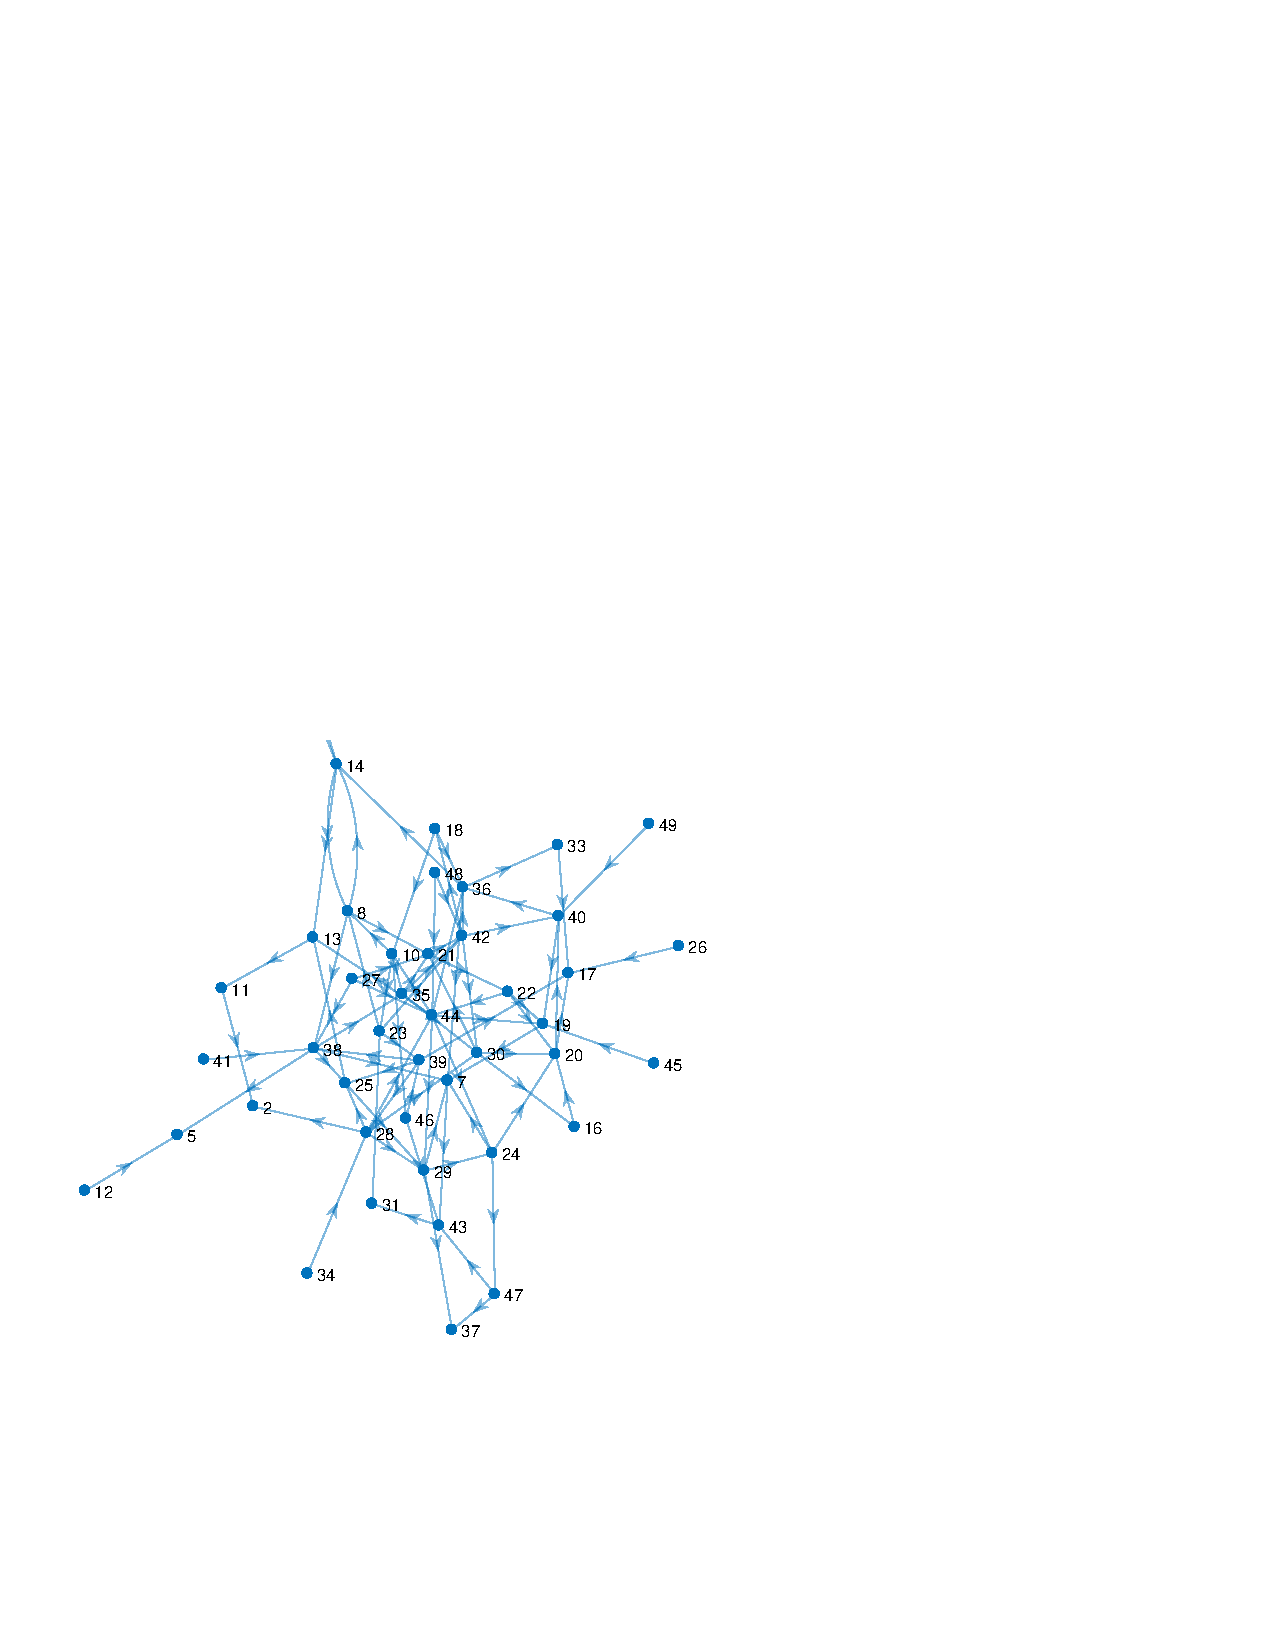
\includegraphics[width=0.8\linewidth]{dag}
%\caption{A Directed Acyclic Graph of the Running AUTOSAR Software Application, Runnables = 50, Paths = 35, Activation Patterns shown in Table \ref{tbl_requirements}.}
%\label{fig_application}
%\end{figure}
%\begin{center}
%\small
%\begin{minipage}{.5\textwidth}%
%\centering
%\begin{tabular}{@{}p{0.25cm}lll@{}}
%\toprule
%C& $r_i$ & $(e_{r_im_1}, e_{r_im_2}, e_{r_im_3})$ & $period$\\ \midrule
%\multirow{4}{4em}{c1} 
%&$r_1$ & (0.030, 0.060, 0.090) & 1\\
%&$r_2$ & (0.041, 0.081, 0.122) & 2\\
%&$r_3$ & (0.083, 0.167, 0.250)  & 5\\ 
%&$r_4$ & (0.310, 0.620, 0.930) & 10 \\[0.3em]
%\hline
%\multirow{2}{4em}{c2} 
%&$r_1$ & (0.310, 0.620, 0.930) & 10\\
%&$r_2$ & (0.310, 0.620, 0.930) & 10\\
%&$r_3$ & (0.310, 0.620, 0.930)  & 10\\ 
%&$r_4$ & (0.310, 0.620, 0.930) & 10 \\[0.3em]
%\hline
%\multirow{2}{4em}{c3} 
%&$r_1$ & (0.310, 0.620, 0.930) & 10\\
%&$r_2$ & (0.291, 0.583, 0.874)) & 10\\
%&$r_3$ & (0.291, 0.583, 0.874)  & 20\\ 
%&$r_4$ & (0.291, 0.583, 0.874) & 20 \\[0.3em]
%\hline
%\multirow{2}{4em}{c4} 
%&$r_1$ & (0.291, 0.583, 0.874) & 20\\
%&$r_2$ & (0.291, 0.583, 0.874)) & 10\\
%&$r_3$ & (0.291, 0.583, 0.874)  & 20\\ 
%&$r_4$ & (0.093, 0.186, 0.279) & 50 \\[0.3em]
%\hline
%\multirow{2}{4em}{c5} 
%&$r_1$ & (0.420, 0.841, 1.261) & 100\\
%&$r_2$ & (0.420, 0.841, 1.261)) & 100\\
%&$r_3$ & (0.420, 0.841, 1.261)  & 100\\ 
%&$r_4$ & (0.420, 0.841, 1.261) & 100 \\[0.3em]
%\bottomrule
%\end{tabular}
%\captionof{table}{Specification of Components.}
%\label{tbl_comps_config}
%\end{minipage}~
%\begin{minipage}{.45\textwidth}
%\begin{center}
%    \begin{tabular}{@{}lll@{}}
%    \toprule
%    Activation, $AP$ & Share & Time, ms \\ \midrule
%    $\tau_1$ & 50  & 50\\
%    $\tau_1\rightarrow\tau_2$ & 20  & 100\\
%    $\tau_1\rightarrow\tau_2\rightarrow\tau_3$ & 20  & 200\\
%    $\tau_1\rightarrow\tau_2\rightarrow\tau_3\rightarrow\tau_4$ & 10  & 400\\
%    \bottomrule
%    \end{tabular}
%    \captionof{table}{Activation Patters of Cause-effect Chains, their Share and End-to-end Timing Requirements.}
%    \label{tbl_requirements}
%\end{center}
%\begin{center}
%    \begin{tabular}{@{}llll@{}}
%    \toprule
%    M  & $P_{idle}$& $P_{busy}$& $\lambda$ \\ \midrule
%    $m_1$ & 50.0& 140.0 &1.0E-3  \\
%    $m_2$ & 10.0& 100.0 &1.0E-4  \\
%    $m_3$ & 10.0& 140.0 &1 .0E-5 \\ \bottomrule
%    \end{tabular}
%    \captionof{table}{Computation Nodes Specification.}
%    \label{tbl_nodes_specification}
%\end{center}
%\end{minipage}
%\end{center}

In the next section, we discuss our proposed method to address the considered optimization problem. 
